\section{Auswertung}
\label{sec:Auswertung}

\subsection{Lange Spule}

Im folgenden wird die magnetische Flussdichte einer langen Spule gemessen und graphisch dargestellt.
%\begin{minipage}{0.5\textwidth}
\begin{table}
\centering
\caption{Messdaten der langen Spule}
\begin{tabular}{c c}
  \toprule
  x (m) &  B (10e-3 T) \\
  \midrule
  -0.02 &         0.23 \\
  -0.01 &         0.28 \\
  -0.01 &         0.35 \\
  -0.01 &         0.46 \\
    0.00 &         0.60 \\
    0.01 &         0.84 \\
    0.01 &         1.15 \\
    0.01 &         1.43 \\
    0.02 &         1.70 \\
    0.03 &         1.89 \\
    0.03 &         2.02 \\
    0.04 &         2.12 \\
    0.04 &         2.18 \\
  \bottomrule
\end{tabular}
\end{table}
%\end{minipage}

%\begin{minipage}{0.5\textwidth}
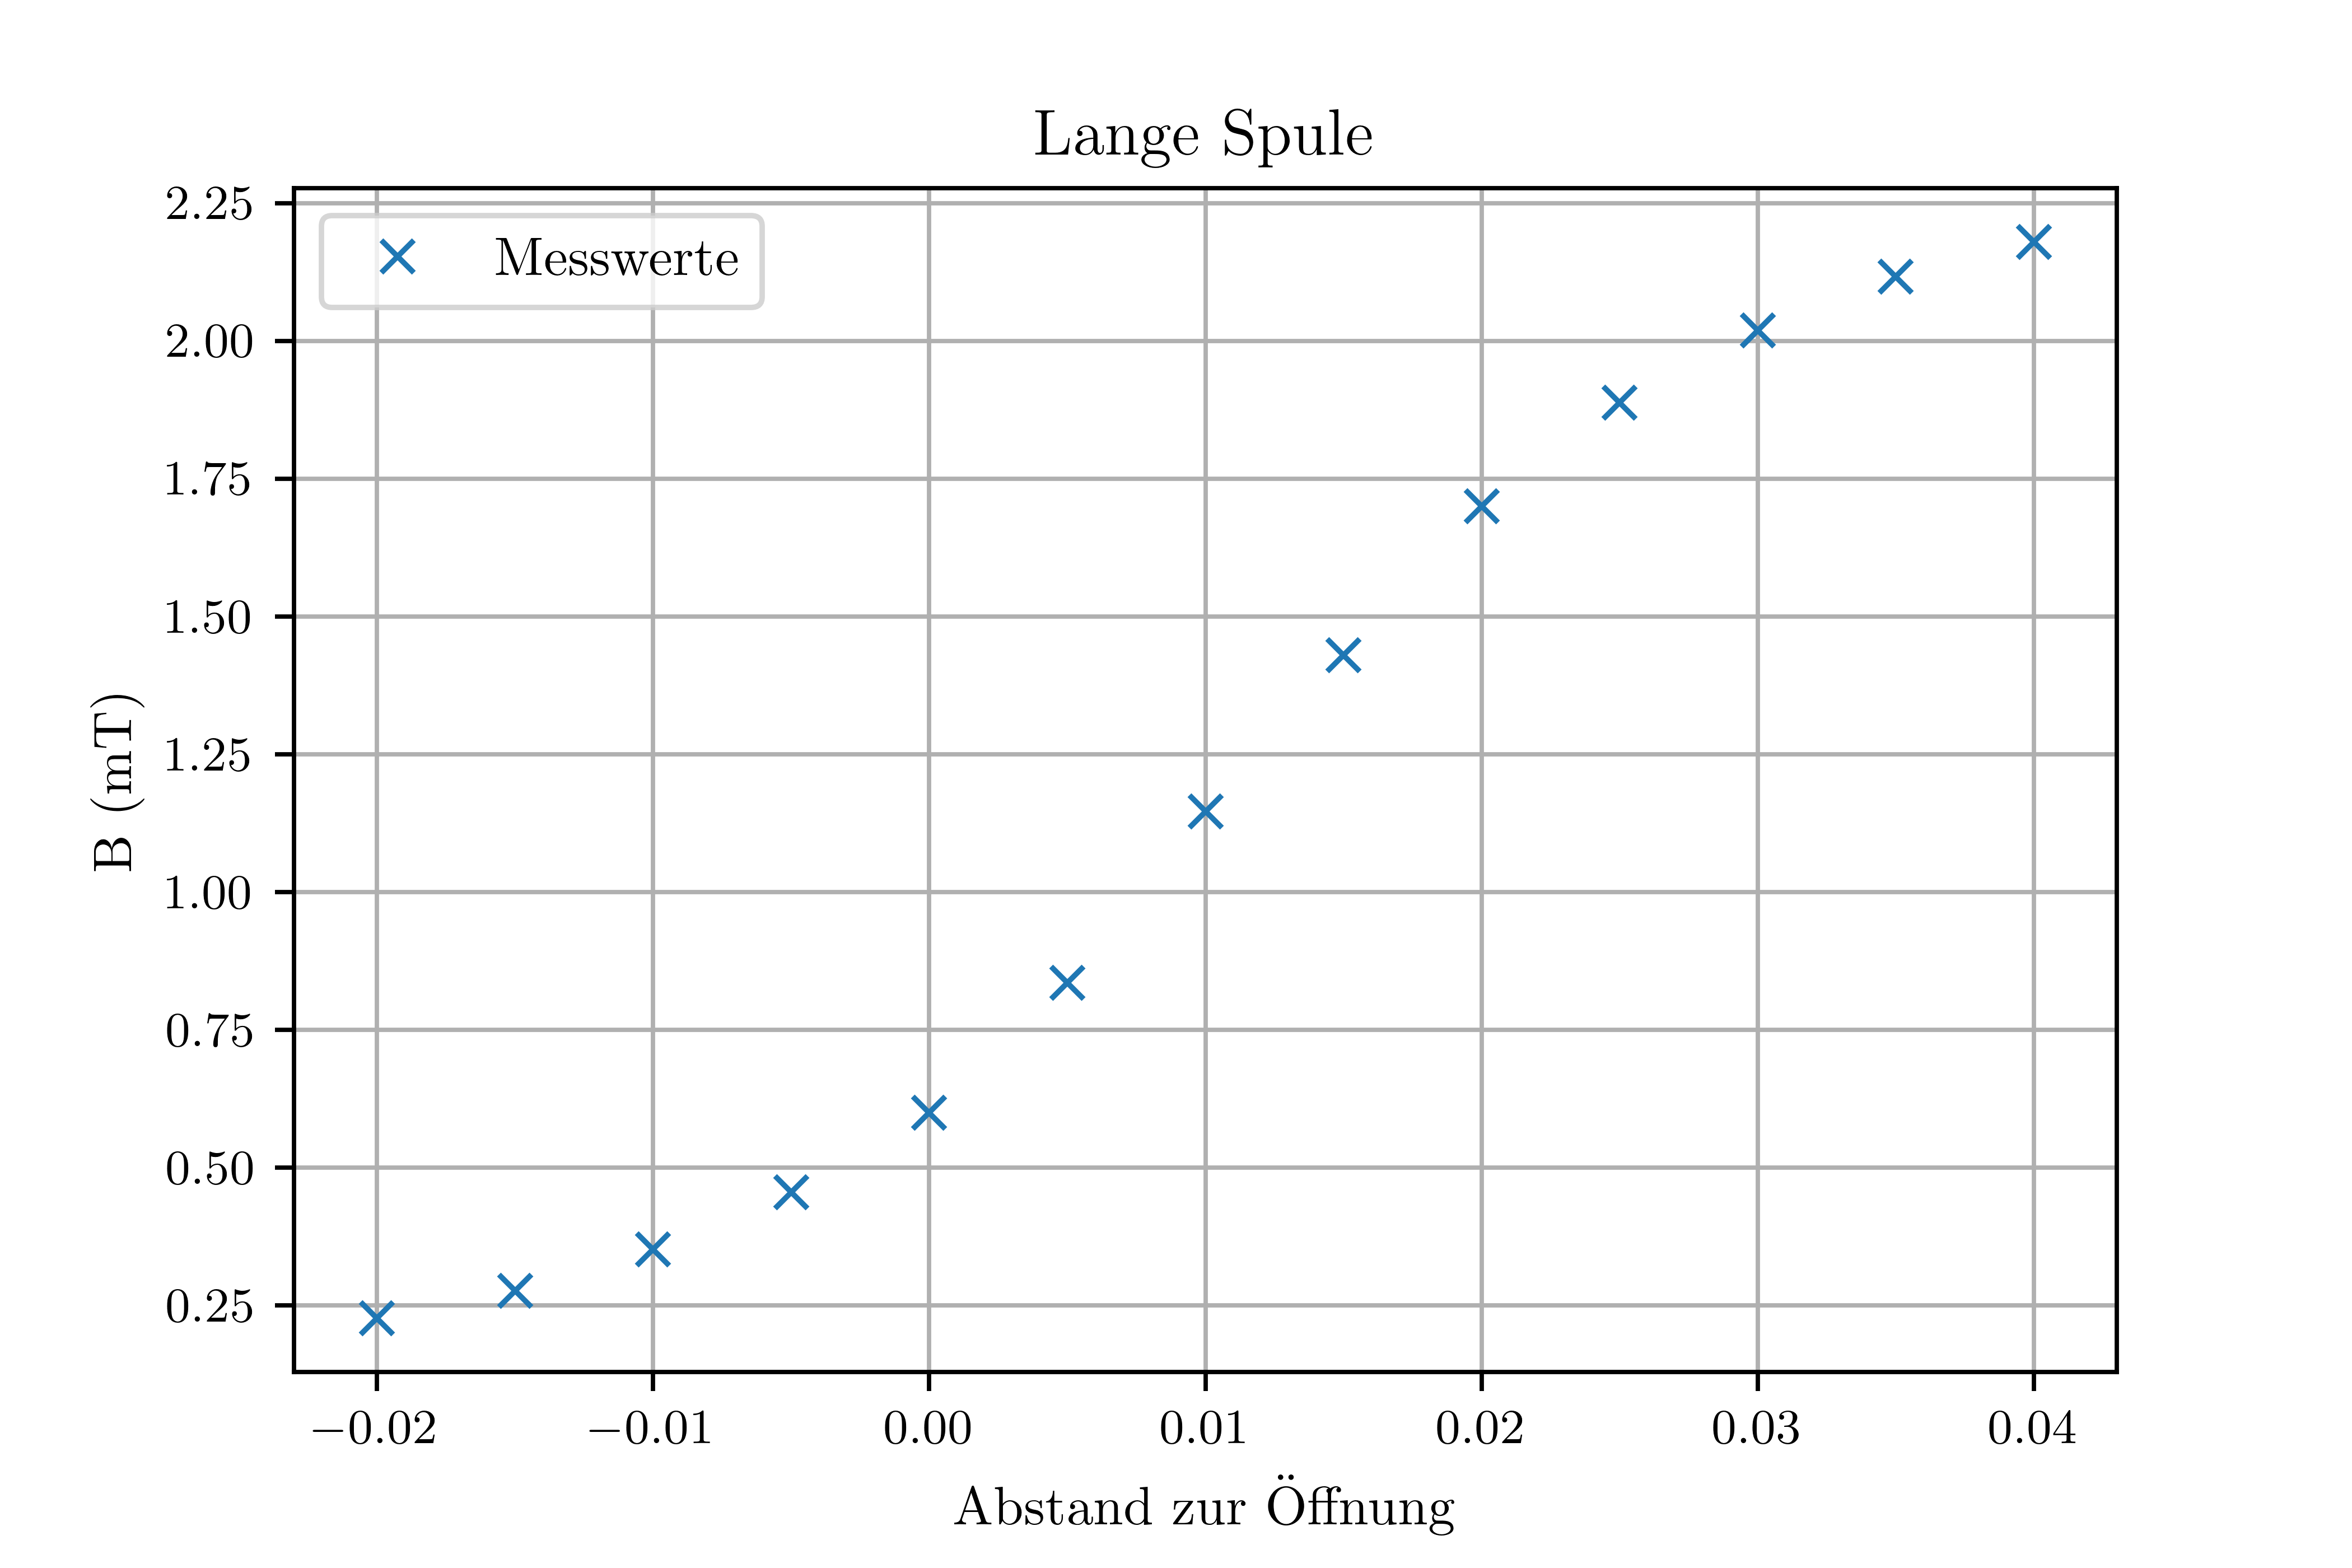
\includegraphics[width=\textwidth]{pictures/LangeSpule1.png}    %Hier fehlt noch die Beschriftung
%\end{minipage}

Es ist eine abflachende Steigung des Magnetfeldes zu erkennen. Der Theoriewert, der sich aus der Formel (\ref{eq:LangeSpule}) ergibt, lautet:
\begin{equation}
  B_{\text{LS}} = 2.31 T
\end{equation}


\subsection{Helmholtzspulenpaar}

Im folgenden sind die Messdaten für die Abstände $d_{1} = 0.012m$, $d_{1} = 0.014m$ und $d_{1} = 0.016m$ in Tabellen und Plots dargestellt.

\begin{table}
\centering
\caption{Messdaten Helmholtzspulenpaar $d_{1} = 0.012m$}
\begin{tabular}{c c}
  \toprule
   x (m) &  B (10e-3 T) \\
  \midrule
  -0.030 &        1.895 \\
  -0.025 &        1.826 \\
  -0.020 &        1.764 \\
  -0.015 &        1.705 \\
  -0.010 &        1.657 \\
  -0.005 &        1.645 \\
   0.000 &        1.632 \\
   0.005 &        1.638 \\
   0.010 &        1.660 \\
   0.015 &        1.700 \\
   0.020 &        1.754 \\
   0.025 &        1.818 \\
   0.030 &        1.890 \\
   0.090 &        1.634 \\
   0.100 &        1.390 \\
   0.110 &        1.137 \\
   0.120 &        0.915 \\
  \bottomrule
\end{tabular}
\end{table}

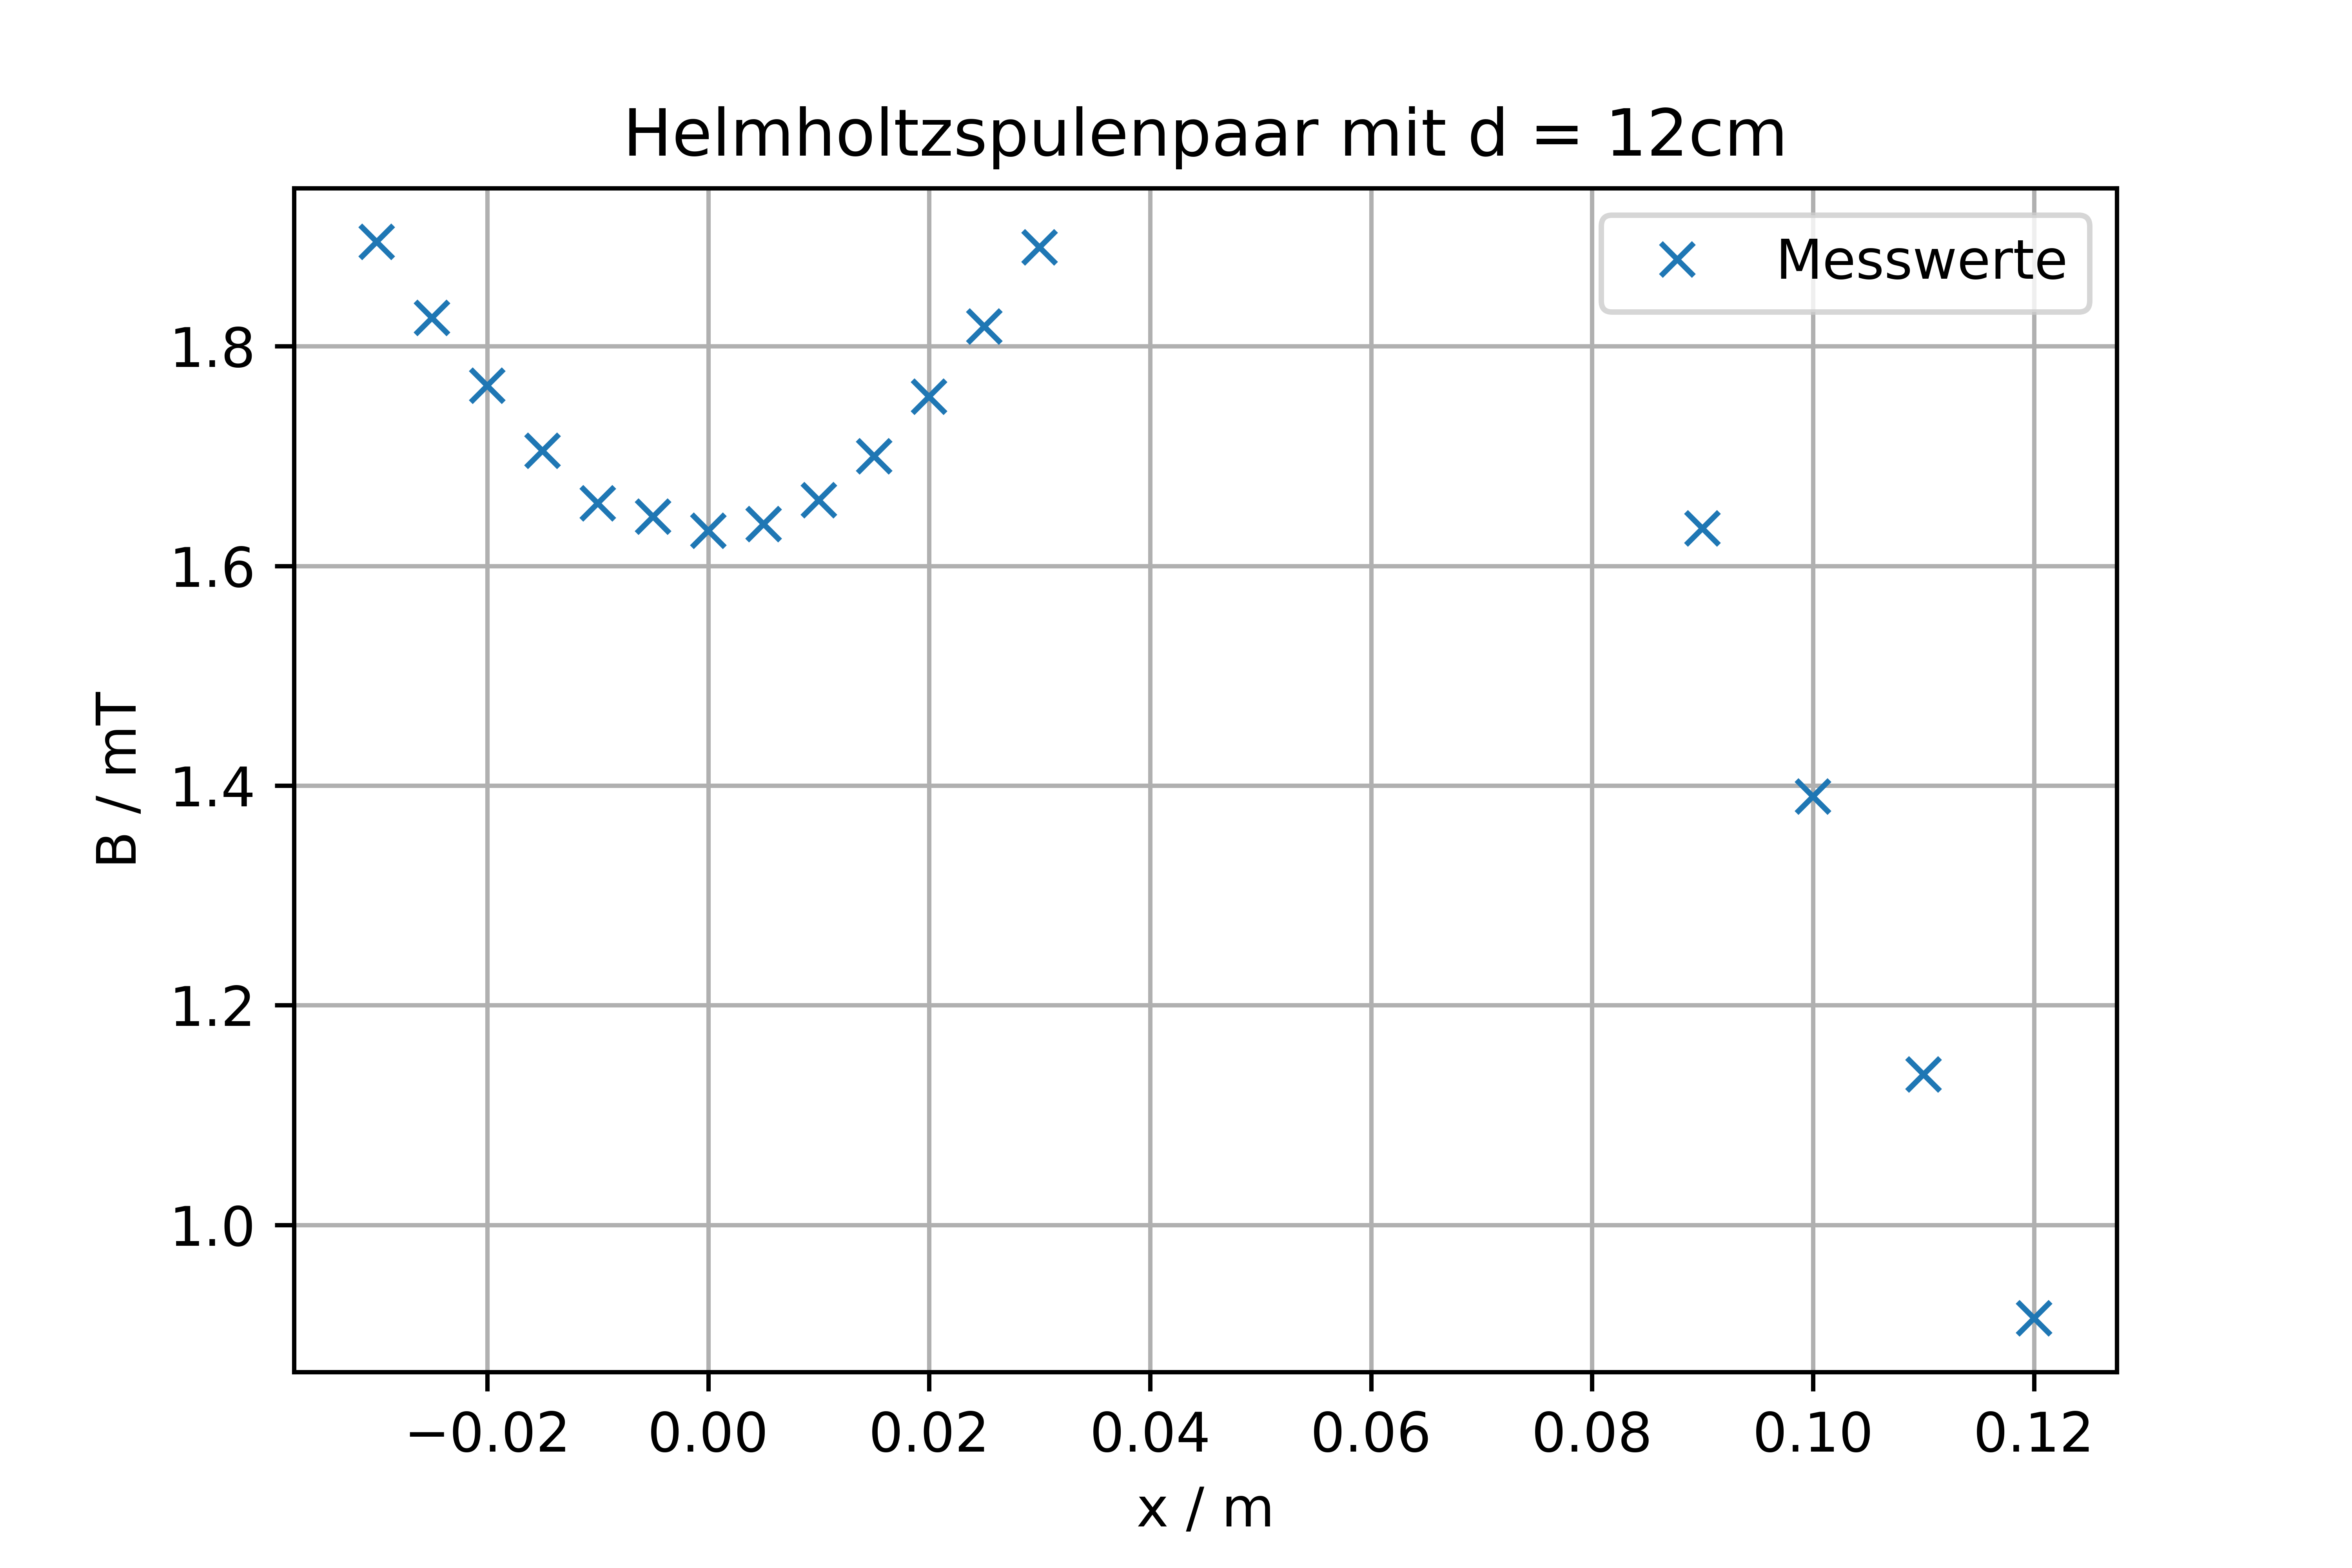
\includegraphics[width=\textwidth]{pictures/Helmholtz1.png}    %Hier fehlt noch die Beschriftung

\begin{table}
\centering
\caption{Messdaten Helmholtzspulenpaar $d_{2} = 0.014m$}
\begin{tabular}{c c}
  \toprule
   x (m) &  B (10e-3 T) \\
  \midrule
  -0.030 &        1.608 \\
  -0.025 &        1.520 \\
  -0.020 &        1.448 \\
  -0.015 &        1.394 \\
  -0.010 &        1.346 \\
  -0.005 &        1.322 \\
   0.000 &        1.312 \\
   0.005 &        1.316 \\
   0.010 &        1.314 \\
   0.015 &        1.375 \\
   0.020 &        1.437 \\
   0.025 &        1.505 \\
   0.030 &        1.572 \\
   0.100 &        1.596 \\
   0.110 &        1.332 \\
   0.120 &        1.091 \\
   0.130 &        0.875 \\
  \bottomrule
  \end{tabular}
\end{table}

\includegraphics[width=\textwidth]{pictures/Helmholtz2.png}    %Hier fehlt noch die Beschriftung


\begin{table}
  \centering
  \caption{Messdaten Helmholtzspulenpaar $d_{3} = 0.016m$}
  \begin{tabular}{c c}
    \toprule
     x (m) &  B (10e-3 T) \\
    \midrule
    -0.030 &        1.300 \\
    -0.025 &        1.225 \\
    -0.020 &        1.160 \\
    -0.015 &        1.112 \\
    -0.010 &        1.074 \\
    -0.005 &        1.054 \\
     0.000 &        1.044 \\
     0.005 &        1.049 \\
     0.010 &        1.073 \\
     0.015 &        1.106 \\
     0.020 &        1.156 \\
     0.025 &        1.210 \\
     0.030 &        1.300 \\
     0.110 &        1.546 \\
     0.120 &        1.295 \\
     0.130 &        1.060 \\
     0.140 &        0.852 \\
    \bottomrule
    \end{tabular}
  \end{table}

  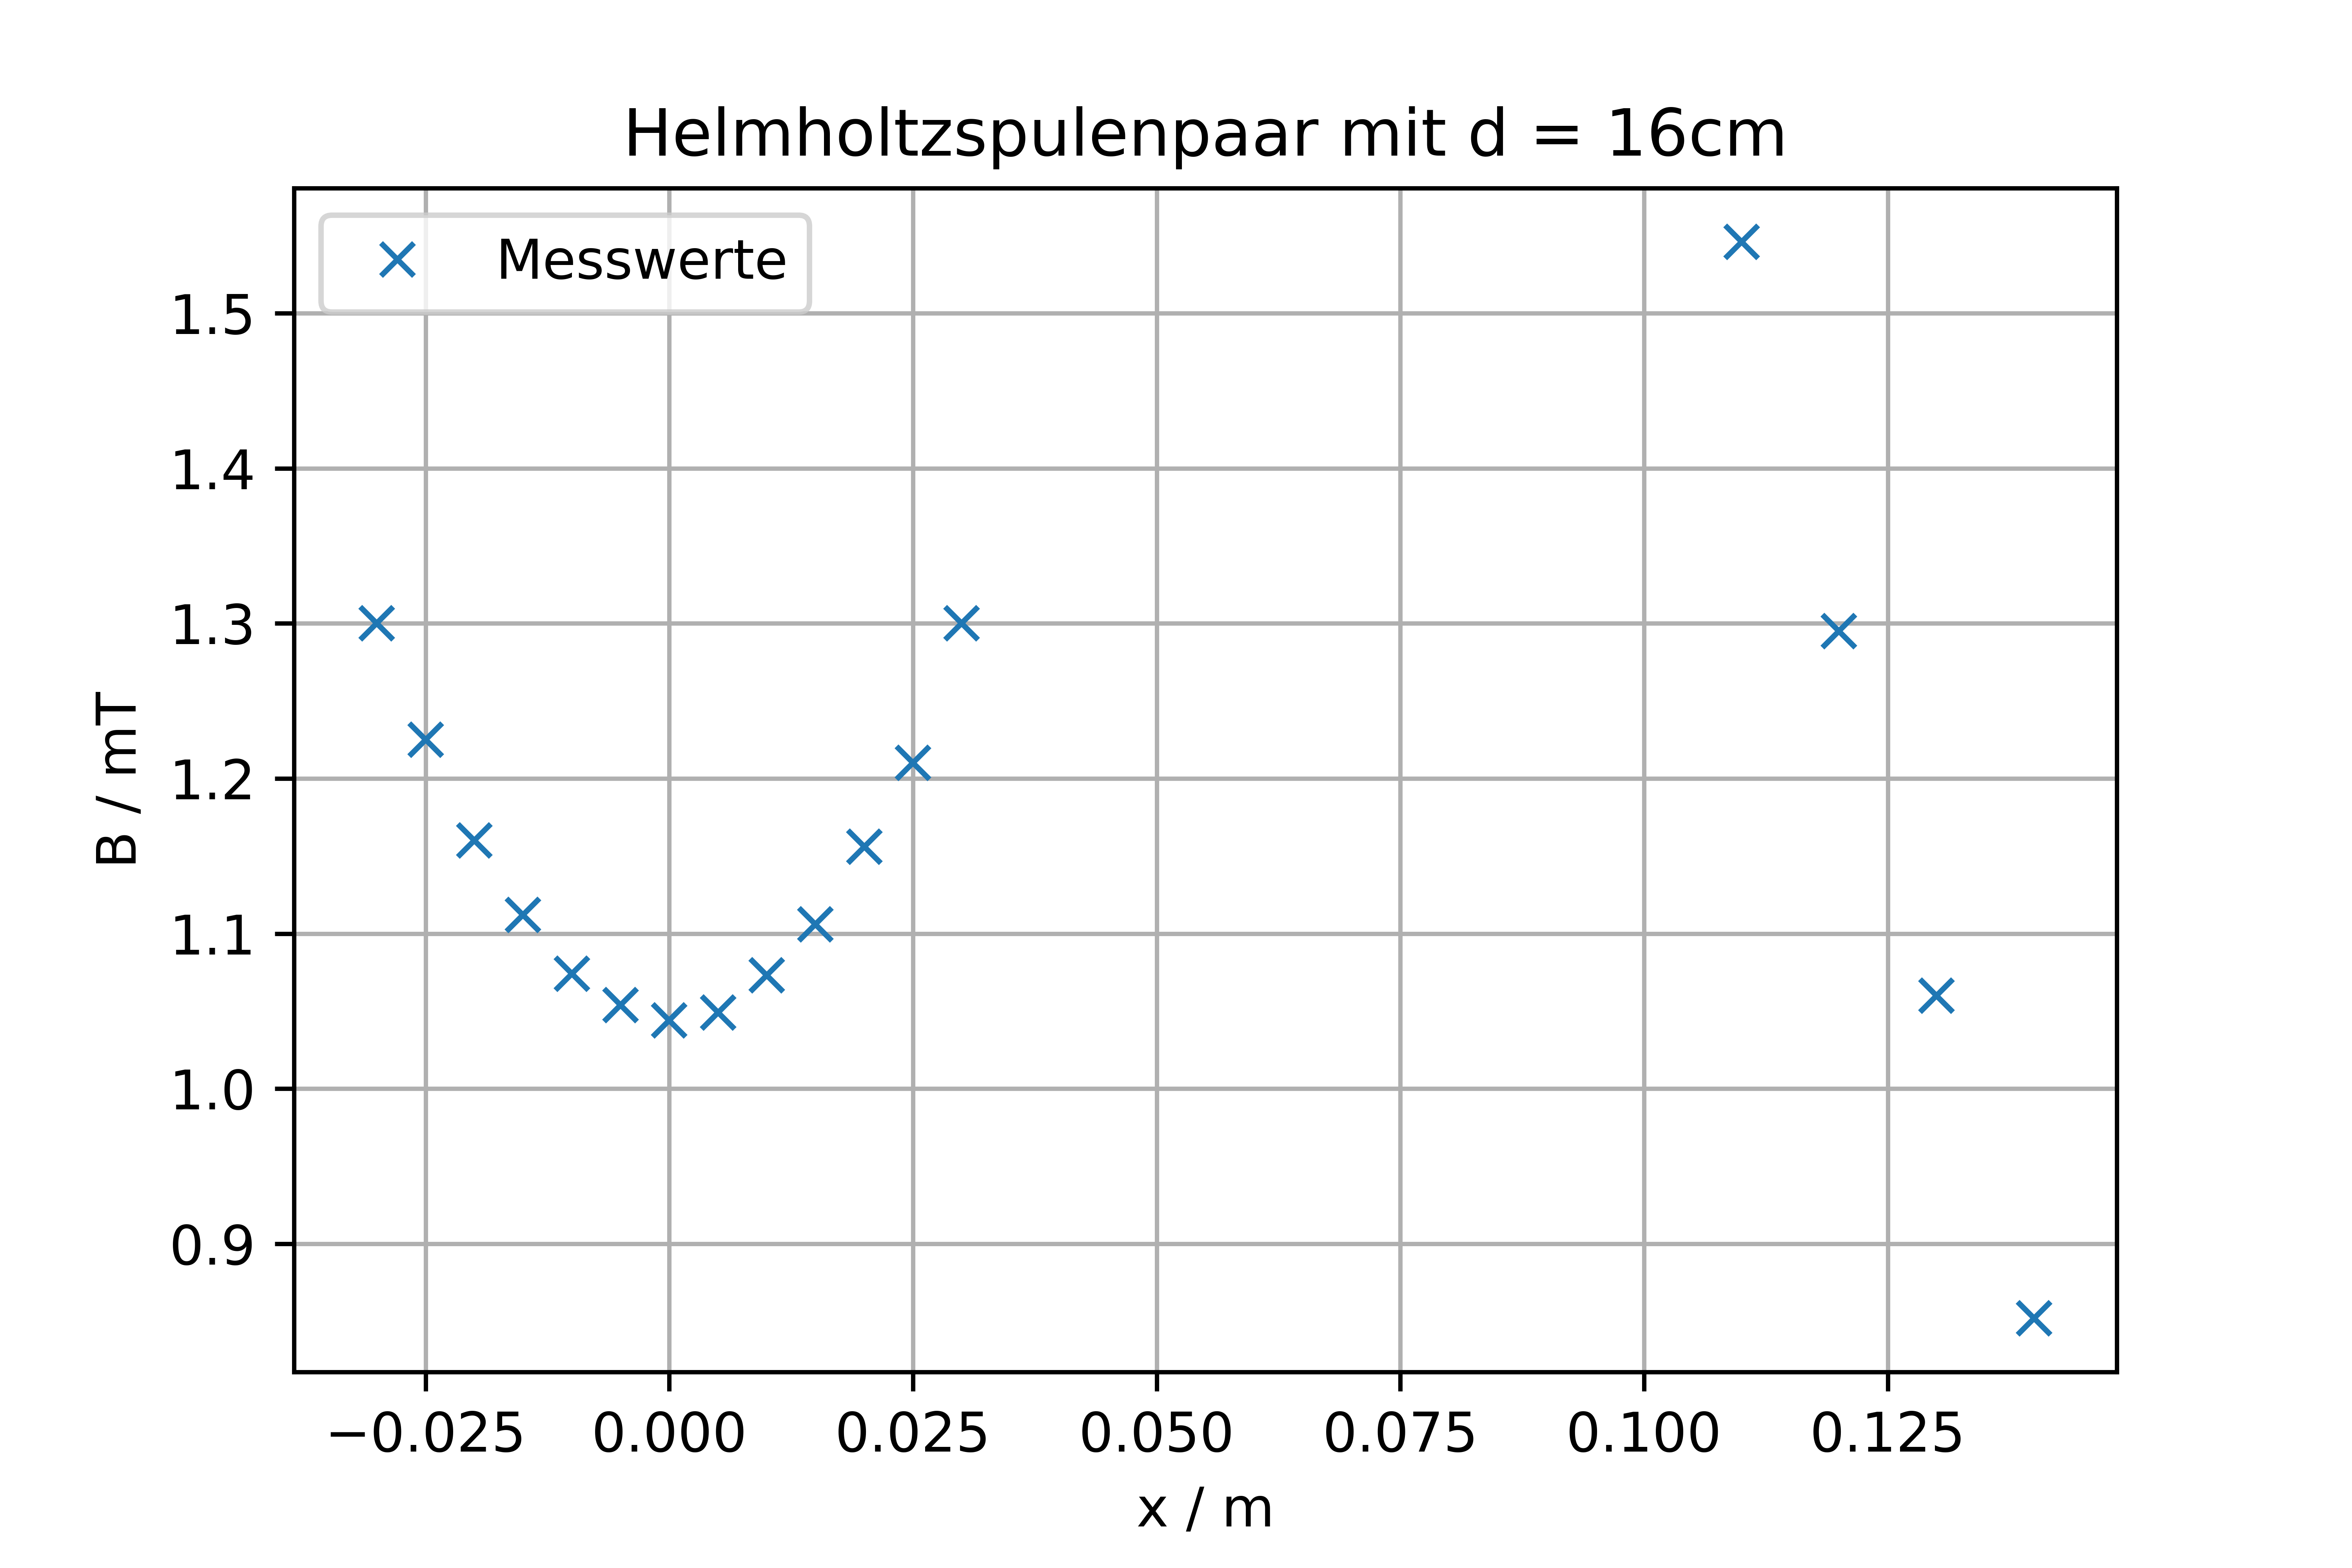
\includegraphics[width=\textwidth]{pictures/Helmholtz3.png}    %Hier fehlt noch die Beschriftung

  Aus Gleichung (\ref{eq:Helmholtzgleichung}) ergeben sich die theoretischen Vergleichswerte.
  In der Tabelle wird das Magnetfeld im Zentrum also mit der Theorie verglichen.

  \begin{table}
    \centering
    \caption{Messdaten der langen Spule}
    \begin{tabular}{c c c c}
      \toprule
      $d_{i}$ & $B_{\text{errech}}$(0) (10e-3T) &  $B_{\text{gemessen}}$(0) (10e-3T) & $\increment$ |$B_{\text{errech}}$(0) - $B_{\text{gemessen}}$(0)| \\
      \midrule
      i = 1  & 1,585 &         1.632  & 0.047  \\ 
      i = 2  & 1.247 &         1.312  & 0.065  \\ 
      i = 3  & 0.985 &         1.044  & 0.059 \\ 
      \bottomrule
    \end{tabular}
    \end{table}